\newpage
\section{Ellipse}
\subsection{Définition bifocale}
\subsubsection{Intersection entre un cylindre et un plan}
\marginpar{\raisebox{-.2ex}{
\includegraphics[height=4ex]{./images/icon/roue.PNG}}\footnotemark[1]}
\footnotetext[1]{Jacques Marot, \url{https://www.geogebra.org/m/yvmuuvx9#material/fsaph7pe}}

\begin{minipage}{0.35\textwidth} % left side: figure
\begin{figure}[H]
    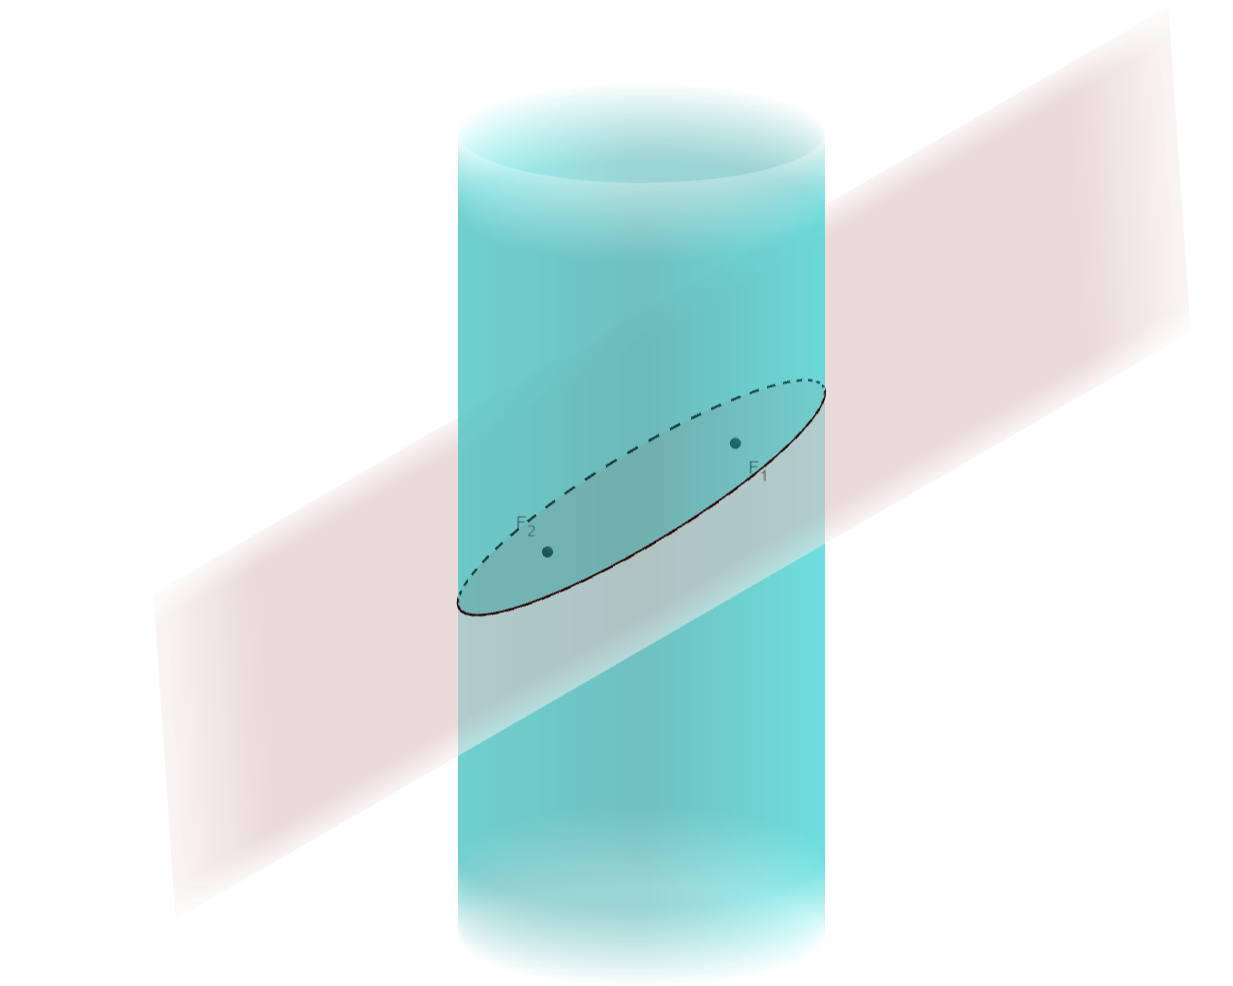
\includegraphics[width = 6cm]{./images/3d/cylindre_ellipse.PNG}
\end{figure}
\end{minipage}
\hfill
\begin{minipage}{0.65\textwidth} % right side: text
Soit le cylindre $\mathcal{C}$ de rayon $r$.\\ 
Lorsque le plan $\Pi$ :
\begin{itemize}
    \item est perpendiculaire à l'axe du cylindre, l'intersection du plan et du cylindre donne un cercle.
    \item est parallèle à l'axe du cylindre, on obtient une droite, deux droites, ou aucune intersection.
    \item n'est ni parallèle, ni perpendiculaire mais a un angle d'inclinaison intermédiaire, 
    l'intersection est ce qu'on appelle une ellipse. C'est-à-dire, soit $\beta$ l'angle entre le plan $\Pi$ et l'axe du cylindre, 
    lorsque $\beta \in ]0; \dfrac{\pi}{2}[$, l'intersection est une ellipse.
\end{itemize} 

\end{minipage}

\vspace{0.5cm}
On étudie ici le dernier cas (elliptique) et les propriétés de cette intersection.
Pour cela, on voudrait à présent inscrire 2 sphères $\mathcal{S}_1, \mathcal{S}_2$ de centres $O_1, O_2$ et de même rayon $r$ dans le cylindre de telle sorte qu'elles soient toutes deux tangentes au plan $\Pi$ également.

\begin{minipage}{0.45\textwidth} % left side: figure
\begin{figure}[H]
    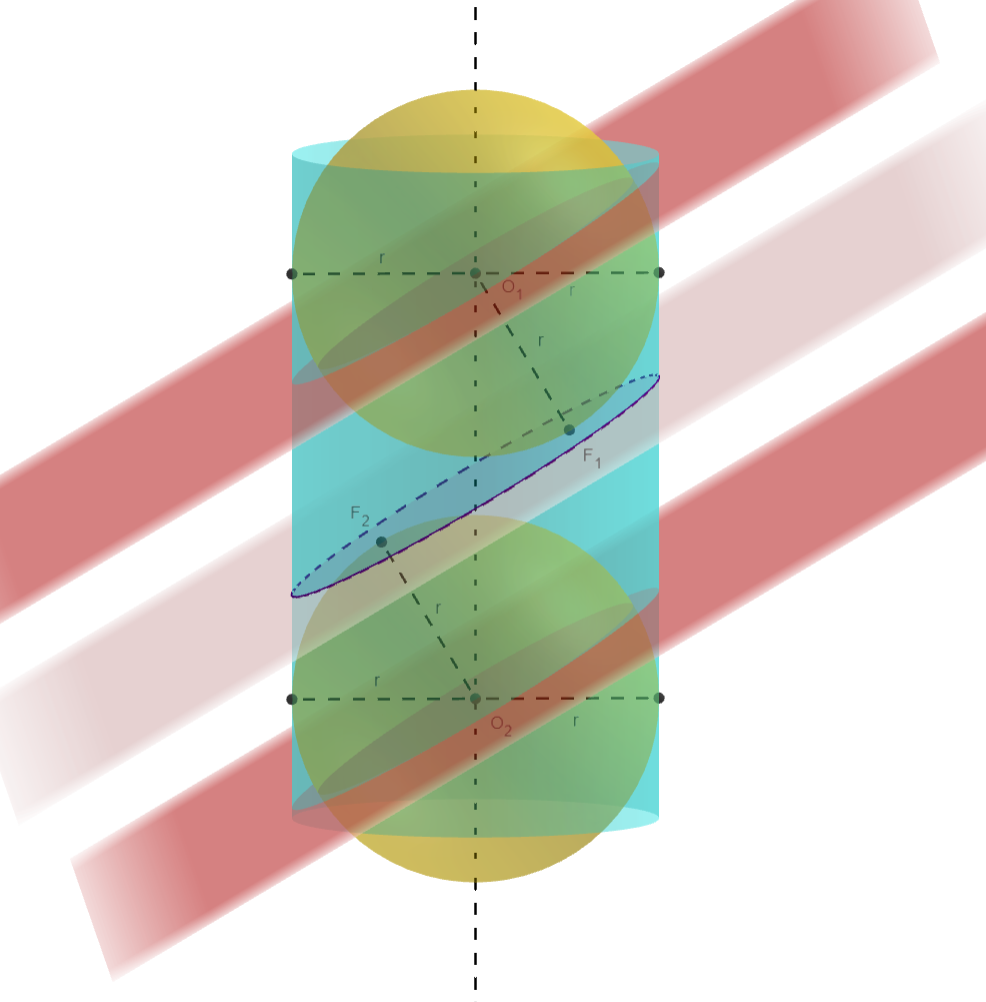
\includegraphics[width = 7cm]{./images/3d/cylindre_e_s_00.PNG}
\end{figure}
\end{minipage}
\hfill
\begin{minipage}{0.5\textwidth} % right side: text
        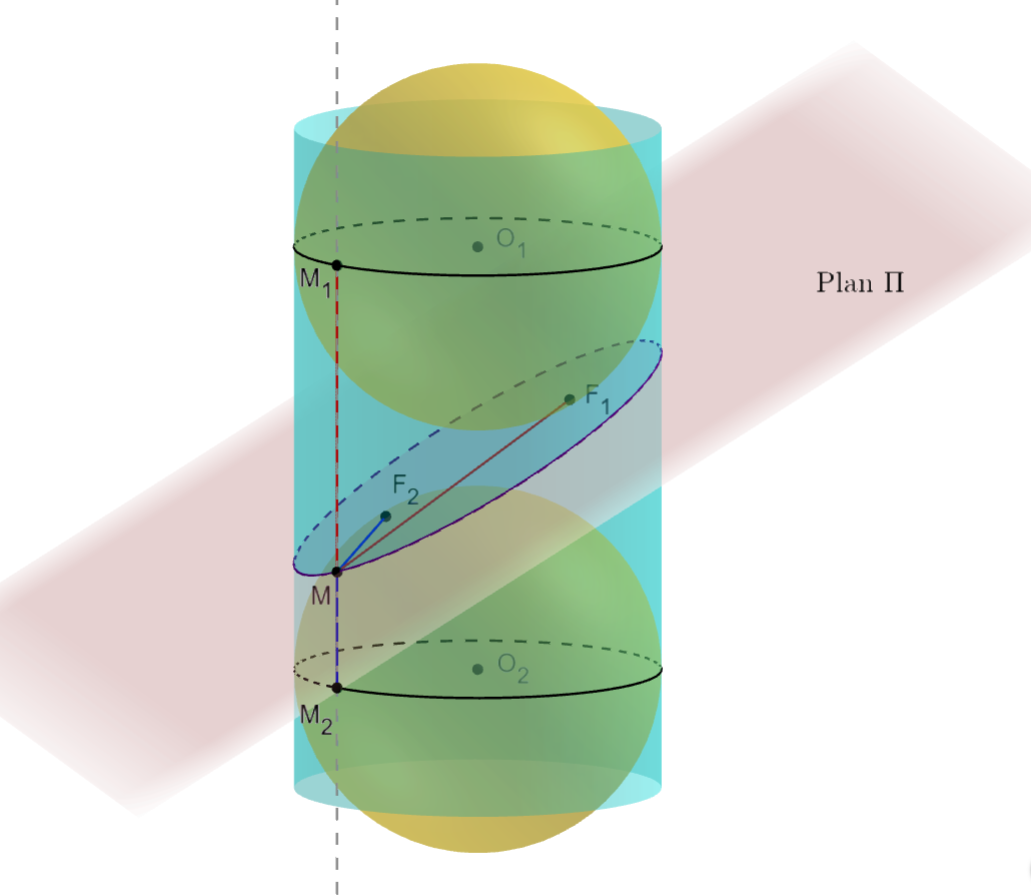
\includegraphics[width = 9cm]{./images/3d/cylindre_ellipse_cst.PNG}
\end{minipage}

A l'aide de 2 plans parallèles à $\Pi$ à une distance $r$ de celui-ci, on détermine les centres $O_1$ et $O_2$ des sphères.\\
Chaque sphère a un point de contact, respectivement $F_1$ et $F_2$, avec le plan $\Pi$.
Soit, $M$ le point d'intersection de $\Pi$ et une génératrice du cylindre. $M_1$ et $M_2$ sont les points de contact entre cette génératrice et les deux sphères. 
Comme les droites $MF_1$ et $MM_1$ sont toutes deux tangentes à la sphère $\mathcal{S}_1$ et toutes deux issues de $M$, par le lemme \ref{lemme_c_s}, on a $\overline{MF_1} = \overline{MM_1}$.\\
De la même manière avec $\mathcal{S}_2$, on a également $\overline{MF_2} = \overline{MM_2}$.\\
On obtient :

\begin{equation}
   \overline{MF_1}+\overline{MF_2}=\overline{MM_1}+\overline{MM_2} = \overline{M_1M_2} = \overline{O_1O_2}
\end{equation}
Comme la distance $\overline{O_1O_2}$ est une constante, on obtient que la somme des distances du point $M$ aux 2 points de contacts $F_1$ et $F_2$ est constante.

\normalcolor
\subsubsection{Intersection entre un cône et un plan}
\marginpar{\raisebox{-.2ex}{
\includegraphics[height=4ex]{./images/icon/roue.PNG}}\footnotemark[2]}
\footnotetext[2]{Jacques Marot, \url{https://www.geogebra.org/m/yvmuuvx9#material/jkubyjmd}}
\begin{minipage}{0.4\textwidth}
    \begin{figure}[H]
    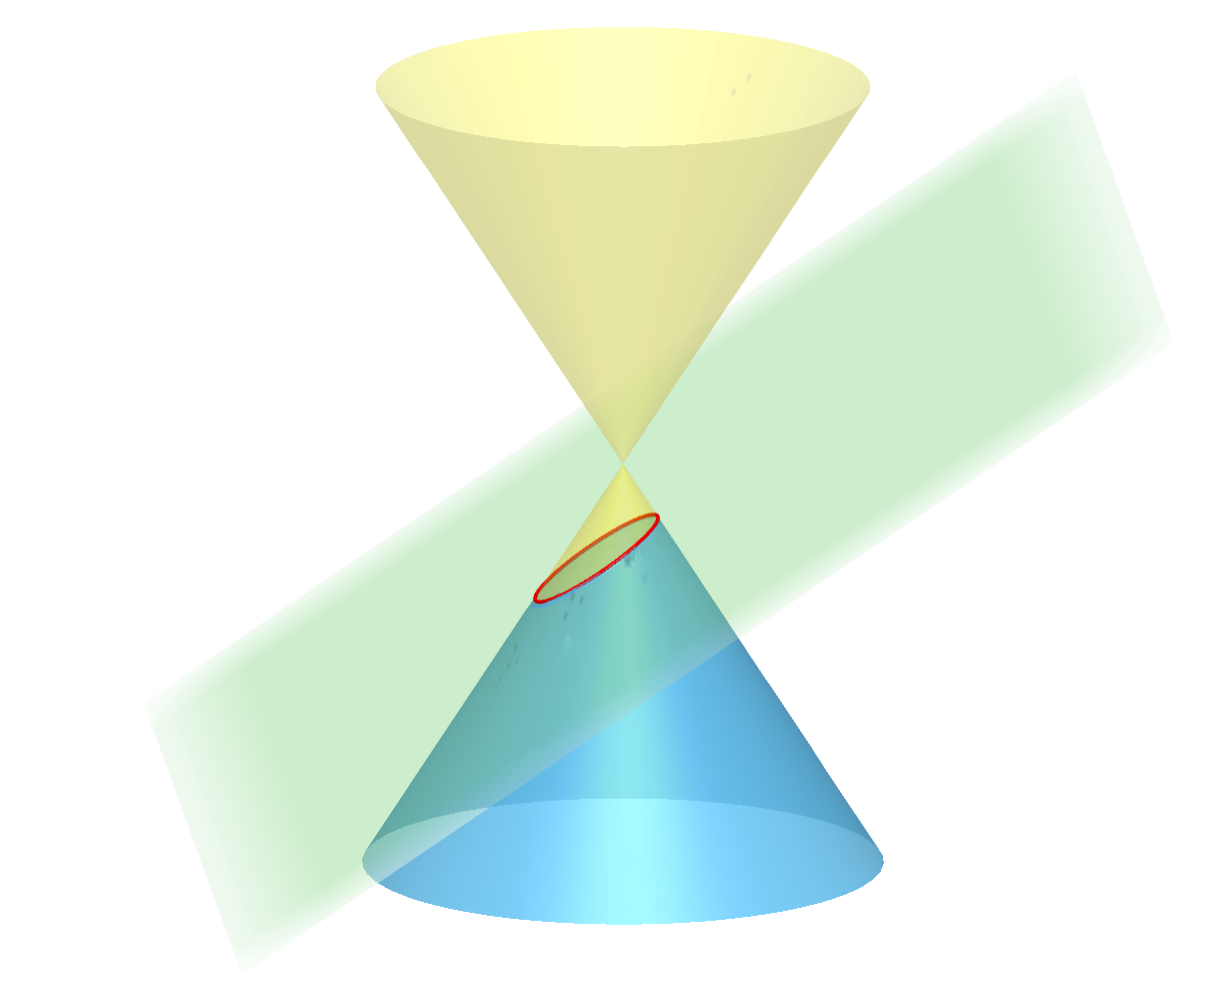
\includegraphics[height=5cm]{./images/3d/cone_ellipse.PNG}
\end{figure}
\end{minipage}
\hfill
\begin{minipage}{0.6\textwidth} % right side: text
    Soient le cône $\mathcal{C}$ de sommet $V$,\\
    $\alpha \in ]0; \dfrac{\pi}{2}[$, l'angle entre une génératrice et l'axe du cône\\
    et $\beta \in [0; \dfrac{\pi}{2}]$, l'angle entre le plan $\Pi$ et l'axe du cône.\\ 
Lorsque $\beta > \alpha$, l'intersection entre le cône et le plan est 
\begin{itemize}
    \item une ellipse
    \item ou dans le cas dégénéré, un point lorsque $\Pi$ passe par le sommet $V$. 
\end{itemize} 
\end{minipage}
On s'intéresse aux propriétés de cette intersection elliptique. Pour cela, de la même manière que pour le cylindre, 
on souhaite à présent inscrire deux sphères $\mathcal{S}_1$ et $\mathcal{S}_2$, de centres $O_1$ et $O_2$ et de rayons $R_1$ et $R_2$, dans le cône $\mathcal{C}$, de sorte qu’elles soient toutes deux tangentes au plan $\Pi$.

Pour qu’une sphère soit à la fois tangente au plan $\Pi$ et aux génératrices du cône, son centre doit être équidistant du plan $\Pi$ et de toutes les génératrices du cône.
Or, le lieu des points équidistants de toutes les génératrices du cône est l’axe du cône. Les centres $O_1$ et $O_2$ doivent donc nécessairement appartenir à cet axe.
Il suffit alors de déterminer, sur cet axe, les points qui sont à la même distance du plan $\Pi$ et des génératrices du cône.\\
\begin{minipage}{0.6\textwidth}
    \begin{figure}[H]
    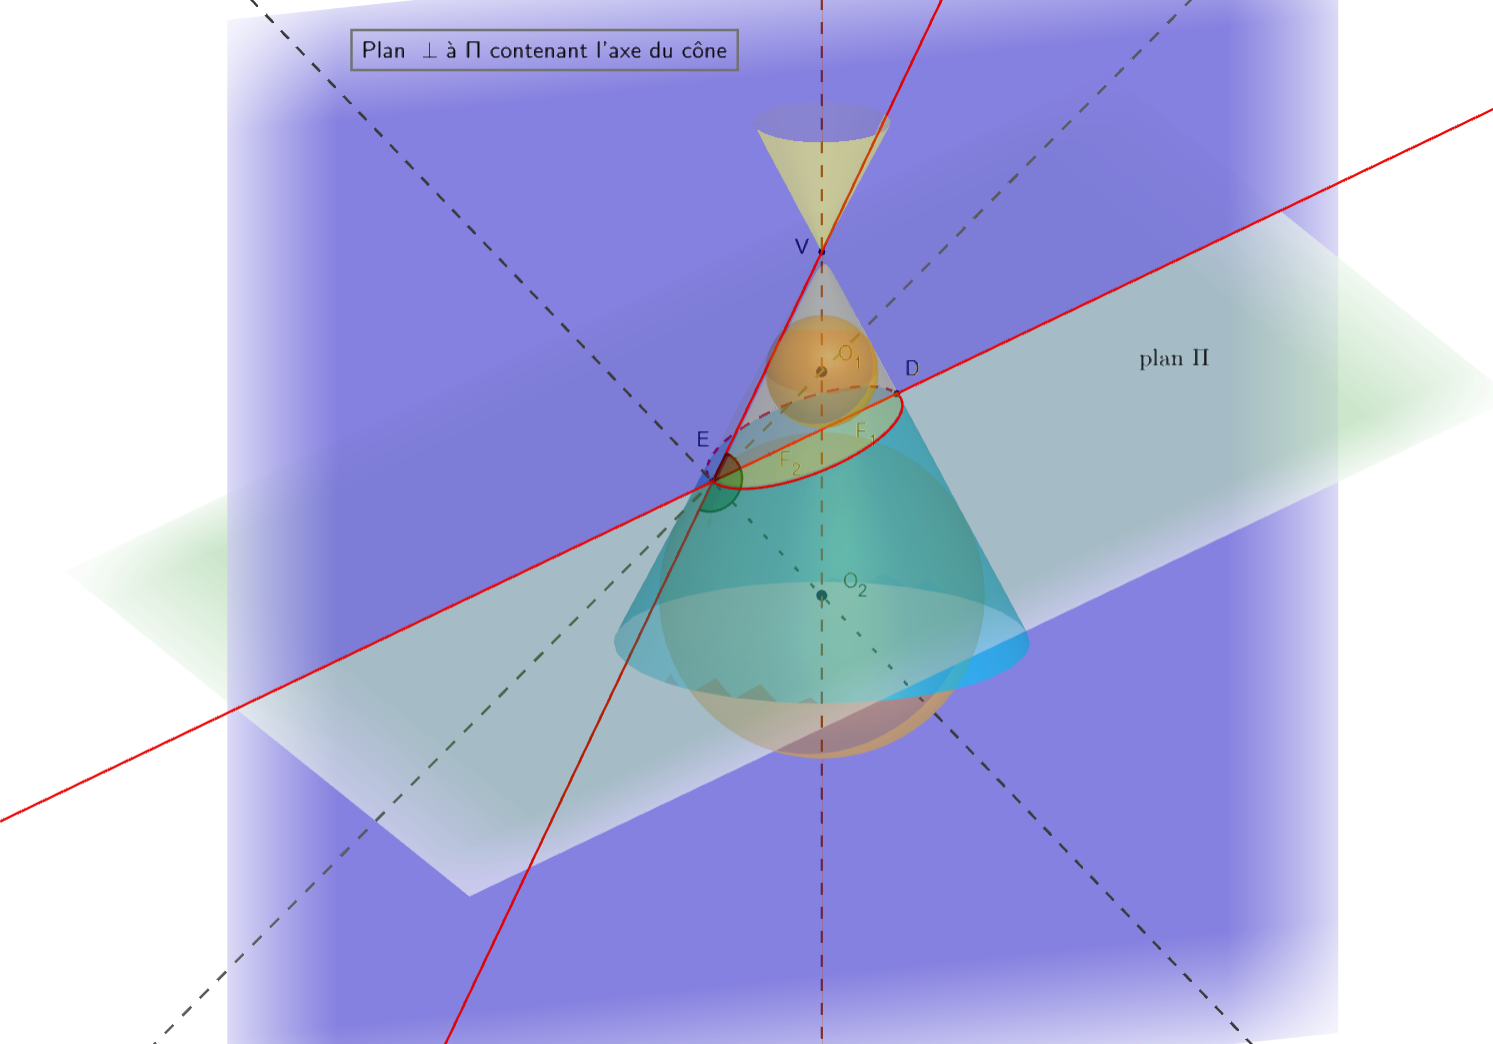
\includegraphics[height=7cm]{./images/3d/cone_sp_2pl.PNG}
\end{figure}
\end{minipage}
\hfill
\begin{minipage}{0.4\textwidth} % right side: text
Pour cela, on se place dans le plan perpendiculaire à $\Pi$ contenant l’axe du cône. Ce plan coupe le cône suivant deux génératrices $(VE)$ et $(VD)$.
Dans ce plan, les points équidistants des droites $(VE)$ et $(ED)$ sont situés sur les bissectrices intérieure et extérieure des angles formés par ces deux droites. Ces bissectrices coupent l’axe du cône en deux points, notés $O_1$ et $O_2$.
\end{minipage}
\vspace{0.5cm}

Par construction, ces points sont équidistants du plan $\Pi$ et des génératrices $(VE)$ et $(VD)$, et donc, par symétrie de révolution du cône, équidistants de toutes les génératrices du cône.
On peut ainsi construire les deux seules sphères tangentes au plan $\Pi$ et inscrites dans le cône, de centres $O_1$ et $O_2$.
Par le lemme \ref{lemme_cercle}, les points de contact de ces sphères avec le cône forment deux cercles $\Gamma_1$ et $\Gamma_2$, de centre $C_1, C_2$, situés respectivement dans des plans $\Pi_1$ et $\Pi_2$ perpendiculaires à l’axe du cône.
Toute génératrice du cône est alors tangente aux deux sphères en des points $M_1$ et $M_2$ appartenant aux cercles $\Gamma_1$ et $\Gamma_2$.\\
De plus, cette génératrice coupe le plan $\Pi$ en un point $M$, qui est l’extrémité commune de quatre segments tangents aux deux sphères : $[MF_1], [MM_1]$ tangents à $\mathcal{S}_1$ et $[MF_2], [MM_2]$ tangents à $\mathcal{S}_2$.
Par le lemme \ref{lemme_c_s}, on a alors : $\overline{MF_1}=\overline{MM_1}$ et $\overline{MF_2}=\overline{MM_2}$. On obtient alors :
\begin{equation}
    \overline{MF_1}+\overline{MF_2}=\overline{MM_1}+\overline{MM_2}=\overline{M_1M_2}=\overline{C_1C_2}.
\end{equation}
La distance $\overline{C_1C_2}$ est constante (ne dépend pas du point $M$). 
Elle dépend de $\overline{O_1O_2}$ et de $\alpha$. $\overline{O_1O_2}$ dépend de l'inclinaison du plan $\Pi$ par rapport à l'angle d'ouverture du cône.
Et donc, $\overline{C_1C_2}$ ne dépend que de $\alpha$ et $\beta$. Pour une coupe de cône donnée ayant la forme d'une ellipse, la somme des distances des points $M$ de l'intersection aux 2 points $F_1$ et $F_2$ est constante. 
\normalcolor
\normalfont
\begin{figure}[H]
    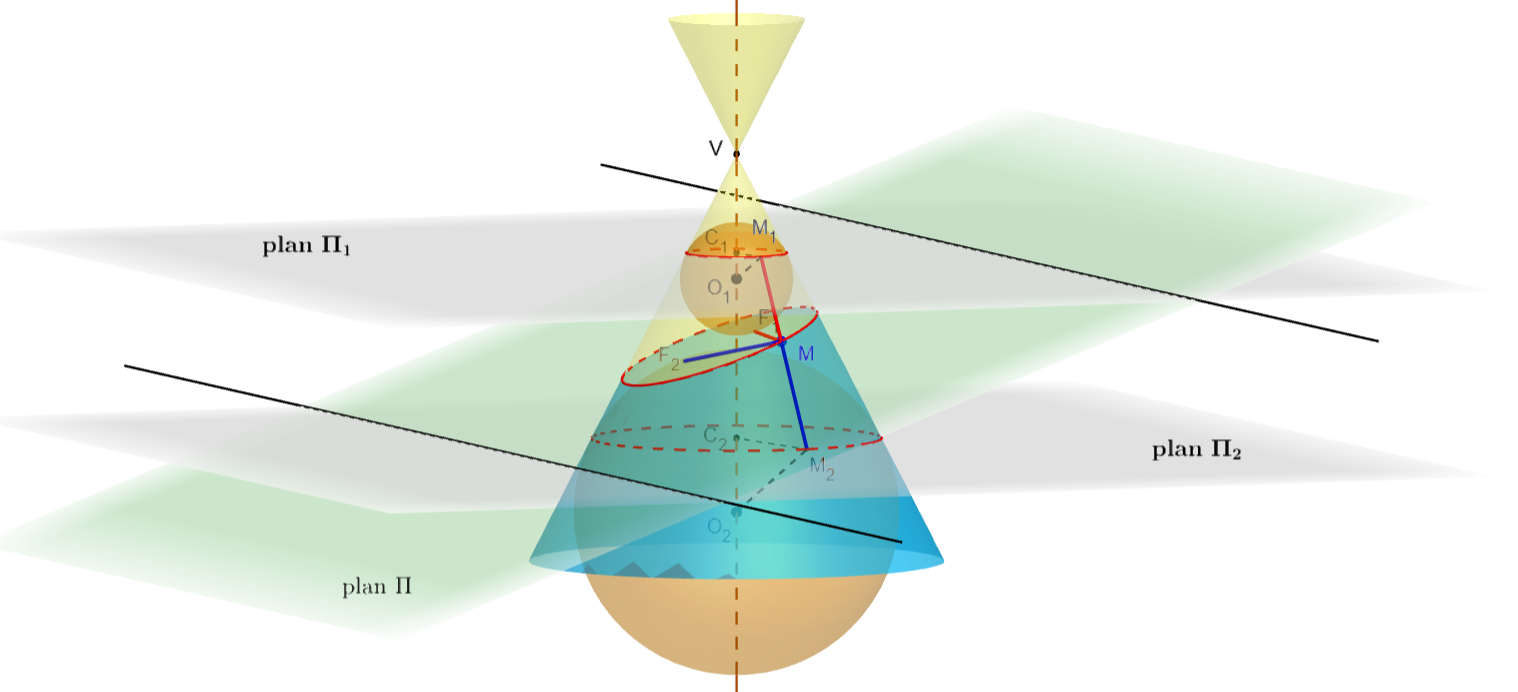
\includegraphics[width = 20cm]{./images/3d/cone_spheres_rot.PNG}
\end{figure}

\thm[Théorème de Dandelin–Quetelet]{
Soit un cône de révolution et un plan ne passant pas par le sommet du cône.
On suppose que ce plan coupe le cône suivant une conique.

Alors :

\begin{itemize}
    \item Il existe une ou deux sphères inscrites dans le cône,
    tangentes à la fois au cône et au plan de coupe.
    
    \item Les points de tangence de ces sphères avec le plan
    sont les foyers de la conique.
\end{itemize}

En particulier :

\begin{itemize}
    \item si la section est une ellipse, il existe deux sphères
    et donc deux foyers ;
    \item si la section est une hyperbole, il existe deux sphères
    et donc deux foyers ;
    \item si la section est une parabole, il existe une seule sphère
    et donc un seul foyer.
\end{itemize}}
\newpage
\subsubsection{Définition bifocale}\label{section:ellbifo}
Nous avons démontré que le lieu de points d'intersection entre un cône $\mathcal{C}$ d'ouverture $2 \alpha$ et un plan $\Pi$ formant un angle $\beta \in ]\alpha;\dfrac{\pi}{2}]$ avec l'axe du cône respecte une propriété de distance à 2 points.\\
Nous nous en inspirons pour définir l'ellipse dans un plan à partir de cette propriété. 
En effet, il est possible de démontrer que toutes les courbes respectant cette propriété peuvent être exprimées comme des sections de cône et que les 2 définitions sont alors équivalentes (théorème de Dandelin-Quetelet).

\begin{tcolorbox}[colback=cyan!5, colframe=cyan!70!blue, title=Définition bifocale de l'ellipse]
\defn{Soient $F_1$ et $F_2$ deux points distincts d’un plan $\Pi$, distants de $\overline{F_1F_2} = 2c$. \\
Une ellipse de foyers $F_1$ et $F_2$ est le lieu des points $M$ du plan $\Pi$ tels que la somme des distances de $M$ à $F_1$ et $F_2$ 
est constante, et strictement supérieure à la distance $\overline{F_1F_2}=2c $.}

\begin{equation}
    \mathcal{E}=\left\{\, M \in \Pi \;\middle|\; 
\overline{MF_1} + \overline{MF_2} = 2a \right\},
\end{equation}


où $a >0 $ est une constante vérifiant $2a > 2c.$
\end{tcolorbox}

\vspace{0.5cm}

\begin{figure}[H]
    \centering
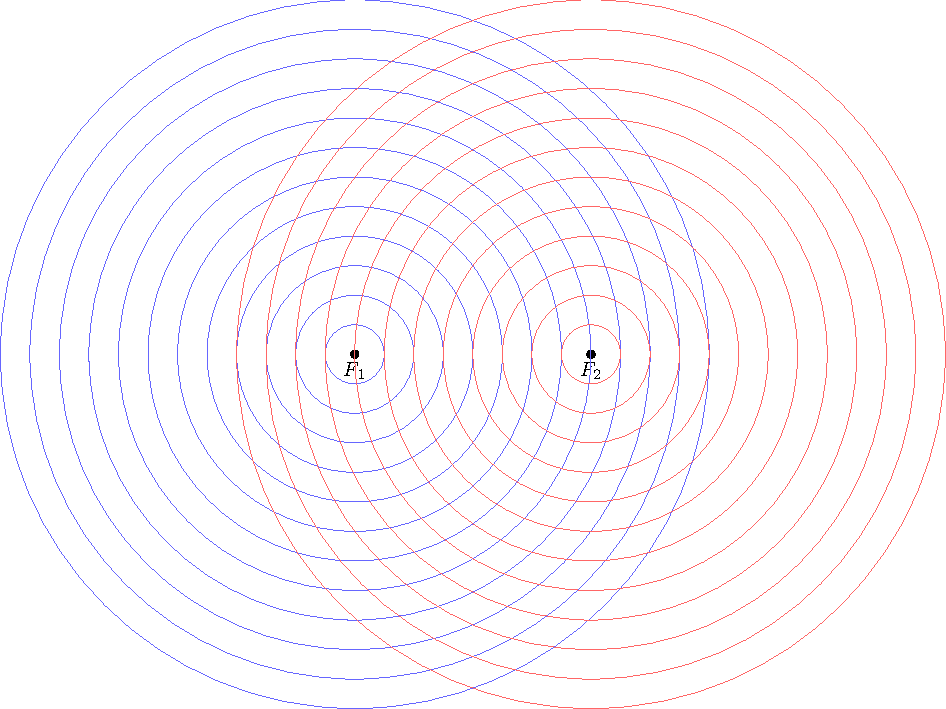
\includegraphics[scale = 0.8]{sections/tikz_standalone/ell_1.pdf}
\end{figure}
\normalfont
A partir de cette définition, tracez une ellipse avec $2a = 11$ unités de longueur.\\
Sans guide tracé, sauriez-vous le refaire avec un compas ?
\newpage
\begin{figure}[H]
\centering
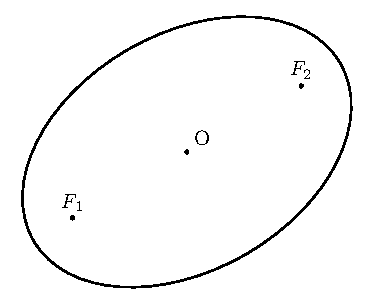
\includegraphics[scale = 1.1]{sections/tikz_standalone/ell_2.pdf}

\end{figure}
\begin{tcolorbox}[colback=cyan!5, colframe=cyan!70!blue, title=Vocabulaire de l'ellipse]

Le \textbf{centre} d'une ellipse est le milieu du segment $[F_1F_2]$ reliant les deux foyers.\\
Un \textbf{diamètre} d'une ellipse est toute droite passant par le centre de l'ellipse.\\
L' \textbf{axe focal} d'une ellipse est la droite $F_1F_2$ passant par les deux foyers.\\ 
L' \textbf{axe non focal} d'une ellipse est l'axe qui est la médiatrice de $[F_1F_2]$.\\ 
La \textbf{distance focale} d'une ellipse est la distance $\overline{F_1F_2} = 2c$ entre les deux foyers.\\
Les \textbf{sommets} $S_1, S_2, S_3, S_4$ d'une l'ellipse sont les points d'intersection de l'ellipse avec ses deux axes.\\
Le \textbf{grand axe} d'une ellipse est le segment de l'axe focal reliant les deux sommets situés sur cet axe. La longueur du grand axe vaut $2a$.\\
Le \textbf{petit axe} d'une ellipse est le segment de l'axe non focal reliant les deux sommets situés sur cet axe. La longueur du petit axe vaut ...\\

\end{tcolorbox}
\newpage 
\begin{tcolorbox}[colback=magenta!5, colframe=red!50!blue, title=Propriétés de l'ellipse]
L'ellipse possède 2 axes de symétries : son axe focal et son axe non focal.\\
L'ellipse possède 1 centre de symétrie : son centre.

\end{tcolorbox}



\begin{minipage}{0.7\textwidth}
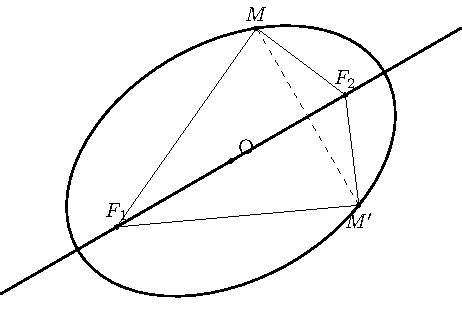
\includegraphics[scale = 1.1]{sections/tikz_standalone/ell_3.pdf}
\end{minipage}
\hfill
\vspace{10pt}
\begin{minipage}{0.7\textwidth}
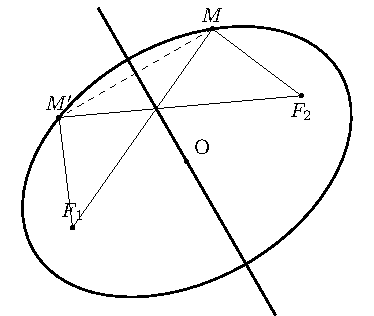
\includegraphics[scale = 1.1]{sections/tikz_standalone/ell_4.pdf}
\end{minipage}
\hfill

\vspace{10pt}
\begin{minipage}{0.7\textwidth}
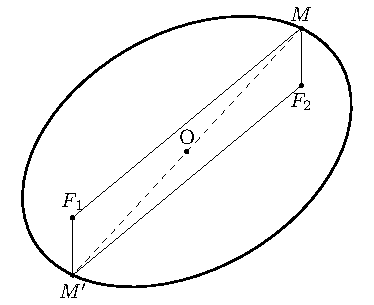
\includegraphics[scale = 1.1]{sections/tikz_standalone/ell_5.pdf}

\end{minipage}
\hfill

\newpage
Choisissons à présent un repère orthonormé commode pour l'étude de l'ellipse :\\
L'axe x est l'axe focal de l'ellipse.\\
L'axe y est l'axe non focal de l'ellipse.
\begin{figure}[H]
\centering

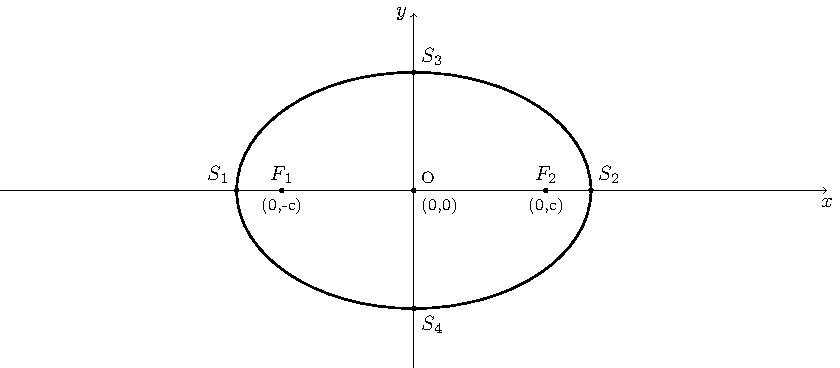
\includegraphics[scale = 1.1]{sections/tikz_standalone/ell_6.pdf}
\end{figure}

\vspace{3cm}
\exo{Exprimez les coordonnées du sommet $S_2$ en fonction des longueurs connues. Déduisez ensuite les coordonnées de $S_1$.}

\newpage

\exo{Exprimez les coordonnées du sommet $S_3$ en fonction des longueurs connues. Déduisez ensuite les coordonnées de $S_4$.}

\begin{eleve}


\vspace{1cm}
\begin{minipage}{0.3\textwidth}
    \begin{align*}
&\overline{S_2F_1} &+& \overline{S_2F_2} &= 2a\\
&c+\overline{OS_2} &+&  \overline{OS_2} -c &= 2a\\
&&&\overline{OS_2} &= a
\end{align*}  
\end{minipage}

\vspace{1cm}

$S_2(a,0)$ et $S_1(-a,0)$

\vspace{1cm}
\begin{minipage}{0.45\textwidth}
    \begin{align*}
\overline{S_3F_1} + \overline{S_3F_2} &= 2a\\
 2\overline{S_3F_2} &= 2a \tag*{(par symétrie)}\\
\overline{S_3F_2} &= a
\end{align*}  
\end{minipage}
\hspace{0.1 \textwidth}
\vrule
\begin{minipage}{0.45\textwidth}
    \begin{align*}
\overline{S_3O}^2 +  \overline{OF_2}^2 &= \overline{S_3F_2}^2 \\
\overline{S_3O}^2 + c^2&= a^2 \\ 
\overline{S_3O}^2 &= a^2 - c^2 >0
\end{align*}  
\end{minipage}

\vspace{1cm}
Posons $b>0$ tel que $b^2 = a^2 - c^2$,\\
$S_3(0,b)$ et $S_4(0,-b)$.
\end{eleve}

\newpage

Repartons à présent de la définition bifocale afin d'obtenir par la méthode de traduction une équation cartésienne dans ce repère choisi.


% Ellipse distance constante
\begin{figure}[H]
\centering
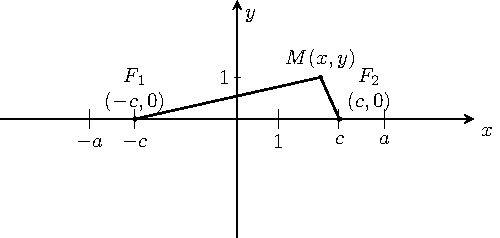
\includegraphics[scale = 1.3]{sections/tikz_standalone/ell_7.pdf}
\end{figure}
\begin{tcolorbox}[colback=white, colframe=green!60!black,  boxrule=0pt, title=Démonstration de l'équation cartésienne de l'ellipse à partir de sa définition bifocale.]
\end{tcolorbox}
\begin{eleve}

    
\begin{align*}
   && \overline{MF_1} + \overline{MF_2} &= 2a\\
    &\iff & \sqrt{(x+c)^2 + y^2} + \sqrt{(x-c)^2 + y^2} &= 2a\\
    &\iff & \sqrt{(x+c)^2 + y^2} &= 2a - \sqrt{(x-c)^2 + y^2}
\end{align*}
Pour éliminer les racines carrées, on peut élever les deux côtés au carré. Cependant, la fonction $x \mapsto  x^2$ n'est pas injective sur $\mathbb{R}$. Le fait de mettre au carré peut faire apparaître des solutions parasites.\\
\begin{align*}
\sqrt{(x+c)^2 + y^2} = 2a - \sqrt{(x-c)^2 + y^2} \notag\\
\iff
\begin{cases}
(\sqrt{(x+c)^2 + y^2})^2 &= (2a - \sqrt{(x-c)^2 + y^2})^2\\[2mm]
2a - \sqrt{(x-c)^2 + y^2} &\ge 0
\end{cases}
\end{align*}

Afin de conserver une équivalence, il faut analyser le signe des membres de l'équation. Le membre de gauche est positif. Il faudra alors s'assurer que le membre de droite l'est aussi.\\
Cette condition $\sqrt{(x-c)^2 + y^2}\leq 2a$ est toujours satisfaite, car par la définition de l'ellipse, la distance $\overline{MF_2}$ ne peut qu'être toujours $< 2a$.
\begin{align*}
    & & \sqrt{(x+c)^2 + y^2} &= 2a - \sqrt{(x-c)^2 + y^2} \notag\\
&\iff&(x+c)^2 + y^2 &= 4a^2 - 4a\sqrt{(x-c)^2 + y^2}+ (x-c)^2 + y^2\\
&\iff& a\sqrt{(x-c)^2 + y^2} &= a^2 - cx
\end{align*}
On peut élever au carré pour éliminer la racine carrée. Il faudra à nouveau faire attention à l'équivalence des équations.\\
Le membre de gauche est positif ($a>0$ et racine carrée). Il faudra alors que le terme de droite soit également positif.\\
\begin{align*}
 a\sqrt{(x-c)^2 + y^2} = a^2 - cx \notag\\
    \iff \begin{cases}
        (a\sqrt{(x-c)^2 + y^2})^2 &= (a^2 - cx)^2\\[2mm]
    a^2 - cx \ge 0
    \end{cases}
\end{align*}

Ainsi, pour que l’équation reste valide, tous les points du lieu doivent avoir une abscisse inférieure ou égale à $\dfrac{a^2}{c}$.
Le point $M (x_{max}, 0)$ , situé le plus à droite sur l’ellipse, correspond au sommet (a,0) calculé précédemment.
Il reste alors à vérifier que $a \leq\dfrac{a^2}{c}$. Ce qui est vérifié, puisque :
\begin{align*}
    c &< a\\
    ac &< a^2 \qquad (\text{car } a>0)\\
    a &< \dfrac{a^2}{c} \qquad (\text{car } c>0)
\end{align*}
On élève alors au carré :
\begin{align*}
a\sqrt{(x-c)^2 + y^2} &= a^2 - cx \notag\\
a^2(x-c)^2 + a^2y^2 &= a^4 - 2a^2cx+c^2x^2\\
(a^2 - c^2)x^2 + a^2y^2 = a^2(a^2-c^2)
\end{align*}
On avait posé précédemment $b^2 = a^2 - c^2$ avec $b>0$. On a alors :
\begin{equation*}
    \mathcal{E} \equiv b^2x^2 + a^2y^2 = a^2b^2
\end{equation*}
\end{eleve}

\newpage
\begin{tcolorbox}[colback=cyan!5, colframe=cyan!70!blue, title=Equation cartésienne réduite de l'ellipse ou équation cartésienne rapportée à ses axes.]
Soit $a, c \in \mathbb{R}^+$ tels que $a > c$.\\
 Dans un repère orthonormé, 
 considérons une ellipse dont les foyers sont $F_1 (-c,0)$ et $F_2 (c,0)$ et dont le grand axe mesure $2a$. Alors son équation cartésienne réduite s'écrit :\\
\begin{equation}
\mathcal{E} \equiv \dfrac{x^2}{a^2} + \dfrac{y^2}{b^2} = 1 \label{eq:EllRed}
\end{equation}
Avec $b^2 = a^2 - c^2$

L' \textbf{excentricité} d'une ellipse est le rapport $\varepsilon = \dfrac{c}{a} \in [0,1[$.\\
\end{tcolorbox}


\vspace{0.5cm}

\begin{minipage}{0.7\textwidth}
    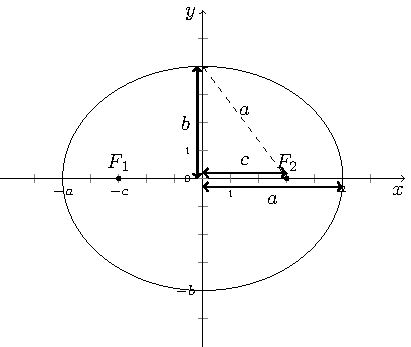
\includegraphics[scale = 1.2]{sections/tikz_standalone/ell_8.pdf}

\end{minipage}
\hfill

\rem{
Que se passe-t-il lorsqu'on fait varier l'excentricité $\varepsilon $ ?\marginpar{\raisebox{-.2ex}{
\includegraphics[height=4ex]{./images/icon/roue.PNG}}\footnotemark[1]}
%Lorsque $a=b$, on trouve l'équation du cercle. En effet, $c=0$, les 2 foyers sont confondus au centre. 
}
\footnotetext[1]{https://www.geogebra.org/graphing/aytm2czt}

\vspace{4cm}
\rem{
Que se passe-t-il si $a=b$ dans l'équation cartésienne? Et si $a<b$ ?\marginpar{\raisebox{-.2ex}{
\includegraphics[height=4ex]{./images/icon/roue.PNG}}\footnotemark[2]} 
%Lorsque $a=b$, on trouve l'équation du cercle. En effet, $c=0$, les 2 foyers sont confondus au centre. 
}
\footnotetext[2]{https://www.geogebra.org/graphing/zmu523gu}

\newpage
\exth{$\dfrac{x^2}{25} + \dfrac{y^2}{9} = 1$.}

\begin{minipage}{0.5\textwidth}
    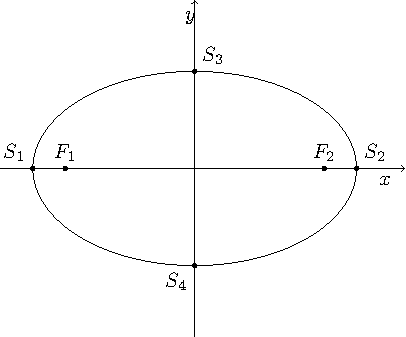
\includegraphics[scale = 1.2]{sections/tikz_standalone/ell_9.pdf}
\end{minipage}
\hfill
\begin{minipage}{0.5\textwidth}
Identifie le centre, l'axe focal, l'axe non focal.\\

Calcule la distance focale, les coordonnées des sommets, la longueur du grand axe et du petit axe.\\
   \begin{eleve}
    Le centre est $(0,0)$\\
    L'axe focal est l'axe des abscisses\\
    L'axe non focal est l'axe des ordonnées\\
    La distance focale est 8 (unités de longueur)\\
    Les sommets sont $S_1(-5,0)$, $S_2(5,0)$, $S_3(0,3)$, $S_4(0,-3)$\\
    Le grand axe est $[S_1S_2]$ et mesure 10 unités de longueur.\\
    Le grand axe est $[S_3S_4]$ et mesure 6 unités de longueur.
    \end{eleve}
\end{minipage}

\vspace{4.5cm}
\exth{Donne l'équation de l'ellipse rapportée à ses axes avec un foyer en (7,0) et une excentricité = 0.5. Esquisse-la.}

\newpage

\exth{On considère un repère orthonormé. Détermine l'équation de l'ellipse de centre (4,7), 
dont l'axe focal est parallèle à l'axe des abscisses et l'axe non focal est parallèle à l'axe des ordonnées. On sait également que son grand axe vaut 18 et sa distance focale vaut 16.
\footnote[1]{Pour plus de détails, voir Changements de repère : Translation, section \ref{section:translation}}}
\newpage
\exth{ Soit une ellipse d'équation:
    $\dfrac{(x-1)^2}{4} + \dfrac{(y+2)^2}{13} = 1$\\
    Identifie le centre, l'axe focal, l'axe non focal.\\
Calcule la distance focale, les coordonnées des sommets, la longueur du grand axe, du petit axe et son excentricité.\\
Esquisse l'ellipse. \footnote[1]{Pour plus de détails, voir Changements de repère : Rotation, section \ref{section:rotation}}
}
\newpage
\subsection{Etude fonctionnelle et graphique}\label{section:ellgraphe}

L'équation de l'ellipse (\ref{eq:EllRed}) n'est pas une équation de fonction.\\
Cependant, il est possible d’étudier sa représentation graphique en la décomposant en deux fonctions correspondant aux parties supérieure et inférieure de l’ellipse :\\
\[f_1 : \mathbb{R} \rightarrow\mathbb{R} : x \rightarrow \dfrac{b}{a}\sqrt{a^2 - x^2} \]
\[f_2 : \mathbb{R} \rightarrow\mathbb{R} : x \rightarrow -\dfrac{b}{a}\sqrt{a^2 - x^2} \]

\exo{Analysez la fonction $f_1$, sa dérivée première, sa dérivée seconde et son graphe.}

\begin{eleve}
\textbf{Etude de $f_1$}\\
Domaine : dom $f_1 = [-a, a]$\\
\\~
Asymptotes ?

$G_{f_1}$ n'admet pas d'asymptote verticale car le domaine est un intervalle fermé.

$G_{f_1}$ n'admet pas d'asymptote horizontale et oblique car le domaine est un intervalle borné. Il n'y a pas de limites en $x\rightarrow +\infty$ et $x\rightarrow -\infty$.\\
\\~
Racines : $G_{f_1}\cap (Ox) = \{(-a,0), (a,0)\}$\\
Ordonnées à l'origine : $G_{f_1}\cap (Oy) = \{(0,b)\}$\\
\\~
Paire: $\forall x \in \text{dom}f_1, f(-x) = \dfrac{b}{a}\sqrt{a^2 - (-x)^2} = f(x)$.\\
On peut se limiter à l'étude de $f_1$ sur $[0,a]$.\\
\\~
Signe de $f_1$ sur $[0,a]$:

$
\begin{array}{c|c c c}
\hline
x & 0 & & a \\
\hline
f(x) & + & + & 
\makebox[1.5cm]{%
  %\color{white!100}\rule{0.5cm}{2cm}
  \raisebox{-0.5\height}{\color{white!50}\rule{0.55cm}{2cm}}
  0
  \raisebox{-0.5\height}{\color{gray!50}\rule{0.85cm}{2cm}}% grey area starts at center
}   \\
\hline
\end{array}
$\\
\\~
\\~
\textbf{Etude de la dérivée première $f'_1$}\\
$f'_1(x) = \dfrac{-bx}{a\sqrt{a^2 - x^2}}$\\
Racines de $f'_1$ : $G_{f'_1}\cap (Ox) = \{(0,0)\}$\\
Signe de $f'_1$ sur $[0,a]$:

$
\begin{array}{c|c c c}
\hline
x & 0 & & a \\
\hline
f'(x) & 0 & - & 
\makebox[1.5cm]{%
  %\color{white!100}\rule{0.5cm}{2cm}
  \raisebox{-0.5\height}{\color{white!50}\rule{0.55cm}{2cm}}
  \raisebox{-0.5\height}{\rule{3pt}{2cm}}% vertical line
  \raisebox{-0.5\height}{\color{gray!50}\rule{0.85cm}{2cm}}% grey area starts at center
}   \\
\hline
\end{array}
$\\
\\~
\\~
\textbf{Etude de la dérivée seconde $f''_1$}\\
$f''_1(x) = \dfrac{-ab}{\sqrt{(a^2 - x^2)^3}}$\\
Racines de $f''_1$ : $G_{f''_1}\cap (Ox) = \{\emptyset\}$\\
Signe de $f''_1$ sur $[0,a]$:

$
\begin{array}{c|c c c}
\hline
x & 0 & & a \\
\hline
f''(x) & - & - & 
\makebox[1.5cm]{%
  %\color{white!100}\rule{0.5cm}{2cm}
  \raisebox{-0.5\height}{\color{white!50}\rule{0.55cm}{2cm}}
  \raisebox{-0.5\height}{\rule{3pt}{2cm}}% vertical line
  \raisebox{-0.5\height}{\color{gray!50}\rule{0.85cm}{2cm}}% grey area starts at center
}   \\
\hline
\end{array}
$\\
\\~
\\~
\textbf{Tableau récapitulatif}\\
$
\begin{array}{c|c c c}
\hline
x & 0 & & a \\
\hline
f'(x) & 0 & - & 
\makebox[1.5cm]{%
  %\color{white!100}\rule{0.5cm}{2cm}
  \raisebox{-0.5\height}{\color{white!50}\rule{0.55cm}{2cm}}
  \raisebox{-0.5\height}{\rule{3pt}{2cm}}% vertical line
  \raisebox{-0.5\height}{\color{gray!50}\rule{0.85cm}{2cm}}% grey area starts at center
}   \\
\hline
f''(x) & - & - & 
\makebox[1.5cm]{%
  %\color{white!100}\rule{0.5cm}{2cm}
  \raisebox{-0.5\height}{\color{white!50}\rule{0.55cm}{2cm}}
  \raisebox{-0.5\height}{\rule{3pt}{2cm}}% vertical line
  \raisebox{-0.5\height}{\color{gray!50}\rule{0.85cm}{2cm}}% grey area starts at center
}   \\
\hline
f(x) & b & \searrow  & 
\makebox[1.5cm]{%
  %\color{white!100}\rule{0.5cm}{2cm}
  \raisebox{-0.5\height}{\color{white!50}\rule{0.25cm}{2cm}}
  0
  \raisebox{-0.5\height}{\color{gray!50}\rule{0.65cm}{2cm}}% grey area starts at center
}   \\
 & & \frown&\\
\hline
\end{array}
$\\
\\~

\end{eleve}

\newpage

\subsection{Définition focale (ou foyer-directrice)}\label{section:ellmonofo}
Jusqu’à présent, nous avons étudié les définitions bifocales des coniques. 
Nous allons maintenant nous intéresser à leurs définitions focales.

Repartons de notre développement de l'équation cartésienne à partir de la définition bifocale de l'ellipse.
\begin{tcolorbox}[colback=white, colframe=green!60!black,  boxrule=0pt, title=Obtention de l'équation focale ou foyer-directrice de l'ellipse à partir de sa définition bifocale.]
\end{tcolorbox}

\begin{eleve}
    \begin{align*}
   && \overline{MF_1} + \overline{MF_2} &= 2a\\
    &\iff & \sqrt{(x+c)^2 + y^2} + \sqrt{(x-c)^2 + y^2} &= 2a\\
    &\iff & \sqrt{(x+c)^2 + y^2} &= 2a - \sqrt{(x-c)^2 + y^2}\\
&\iff&(x+c)^2 + y^2 &= 4a^2 - 4a\sqrt{(x-c)^2 + y^2}+ (x-c)^2 + y^2\\
&\iff& a\sqrt{(x-c)^2 + y^2} &= a^2 - cx\\
&\iff& \sqrt{(x-c)^2 + y^2} &= \dfrac{c}{a}(\dfrac{a^2}{c} - x)\\
&\iff& \sqrt{(x-c)^2 + y^2} &= \dfrac{c}{a}\left\lvert \dfrac{a^2}{c} - x\right\rvert  \tag{$\dfrac{a^2}{c} - x\geq0$ voir \ref{section:ellbifo}}\\
&\iff& \sqrt{(x-c)^2 + y^2} &= \dfrac{c}{a}\left\lvert x - \dfrac{a^2}{c}\right\rvert
\end{align*}

Le terme de gauche de l'équation représente la distance entre un point $M(x,y)$ et le foyer $F_2(c,0)$.\\
Le terme $\left\lvert x - \dfrac{a^2}{c}\right\rvert$ représente la distance entre un point $M(x,y)$ et une droite $d_{F_2} \equiv x = \dfrac{a^2}{c}$.\\
Cette dernière équation exprime donc que le rapport entre la distance d’un point $M(x,y)$ de l’ellipse au foyer $F_2$ 
et la distance de ce point $M$ à la droite $d_{F_2}$, d’équation $x = \dfrac{a^2}{c}$, est constant.\\
\\~
On peut également obtenir une formulation en fonction du foyer $F_1(-c,0)$.\\

On a alors :
\begin{equation}
    (x-c)^2 + y^2 = \varepsilon^2 \left(x - \dfrac{a^2}{c}\right)^2
\end{equation}
\begin{equation}
    (x+c)^2 + y^2 = \varepsilon^2 \left(x + \dfrac{a^2}{c}\right)^2
\end{equation}
\end{eleve}



\newpage
\null
\newpage

\begin{tcolorbox}[colback=cyan!5, colframe=cyan!70!blue, title=Définition focale de l'ellipse]
\defn{Soient 
\begin{itemize}
    \item $F$ un point d'un plan $\Pi$,
    \item $d_F$ un droite de $\Pi$ ne passant pas par $F$,
    \item et une constante $\varepsilon \in [0,1[$
\end{itemize}
une ellipse de foyer $F$, de \textbf{directrice} associée $d_F$ et d'\textbf{excentricité} $\varepsilon$
est le lieu des points $M$ du plan $\Pi$ tels que le rapport des distances de $M$ à $F$ et de $M$ à $d_F$ est constant et égal à $\varepsilon$.}

\[
\frac{d(M,F)}{d(M,d_F)} = \varepsilon,
\]
Dans ce cas, $\varepsilon = \frac{c}{a}$, avec $a$ le demi grand axe de l'ellipse. 

\end{tcolorbox}

\begin{tcolorbox}[colback=cyan!5, colframe=cyan!70!blue, title=Equation focale de l'ellipse rapportée à ses axes.]
Soient $a,c\in\mathbb{R}^+$ tels que $a>c$.

Dans un repère orthonormé, considérons une ellipse de foyers
$F_1(-c,0)$ et $F_2(c,0)$, et de directrices associées
\[
d_{F_1}\equiv x=-\dfrac{a^2}{c},
\qquad
d_{F_2}\equiv x=\dfrac{a^2}{c},
\]

Tout point $M(x,y)$ appartenant à cette ellipse vérifie les deux équations focales équivalentes :
\[
(x-c)^2+y^2=\varepsilon^2\left(x-\dfrac{a^2}{c}\right)^2,
\]
\[
(x+c)^2+y^2=\varepsilon^2\left(x+\dfrac{a^2}{c}\right)^2.
\]

avec l'excentricité $0\le \varepsilon = \dfrac{c}{a}<1$.
\end{tcolorbox}
\clearpage
\thispagestyle{empty}
\begin{center}
\begin{tabular}{|>{\centering\arraybackslash}m{3cm}|>{\centering\arraybackslash}m{7cm}|>{\centering\arraybackslash}m{7cm}|}
    \hline
     Équation & $\dfrac{x^{2}}{a^{2}} + \dfrac{y^{2}}{b^{2}} = 1 \quad (a>b)$ & \\
     \hline
     Lien entre $a$, $b$ et $c$ & $b^{2} = a^{2} - c^{2}$ & \\
     \hline
     Foyers & $(c,0)$ et $(-c,0)$ & \\
     \hline
     Longueur du grand axe & $2a$ & \\
     \hline
     Longueur du petit axe & $2b$ &  \\
     \hline
     Axe focal & Axe $Ox$ &  \\
     \hline
     Sommets & $(-a,0)$, $(a,0)$, $(0,b)$ et $(0,-b)$ &  \\
     \hline
     Directrice &  &  \\
     \hline
     Excentricité & $\varepsilon = \dfrac{c}{a} \qquad (<1)$ &  \\
     \hline
     Schéma & 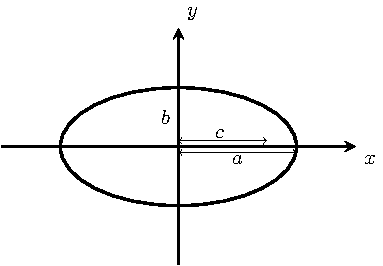
\includegraphics[scale=0.7]{sections/tikz_standalone/ell_10.pdf} & 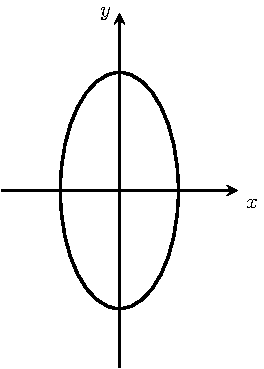
\includegraphics[scale=0.7]{sections/tikz_standalone/ell_11.pdf}\\
     \hline
\end{tabular}
\end{center}
\clearpage
\thispagestyle{empty}
\begin{center}
\begin{tabular}{|>{\centering\arraybackslash}m{3cm}|>{\centering\arraybackslash}m{7cm}|>{\centering\arraybackslash}m{7cm}|}
    \hline
     Équation & $\dfrac{(x-x_c)^{2}}{a^{2}} + \dfrac{(y-y_c)^{2}}{b^{2}} = 1 \quad (a>b)$ & \\
     \hline
     Lien entre $a$, $b$ et $c$ &  & \\
     \hline
     Foyers &  & \\
     \hline
     Longueur du grand axe &  & \\
     \hline
     Longueur du petit axe &  &  \\
     \hline
     Axe focal & droite parallèle à l'axe $Ox$ passant par $(x_c,y_c)$ &  \\
     \hline
     Sommets & &  \\
     \hline
     Directrice &  &  \\
     \hline
     Excentricité &  &  \\
     \hline
     Schéma & 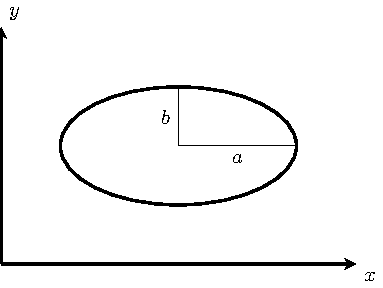
\includegraphics[scale=0.7]{sections/tikz_standalone/ell_12.pdf} & 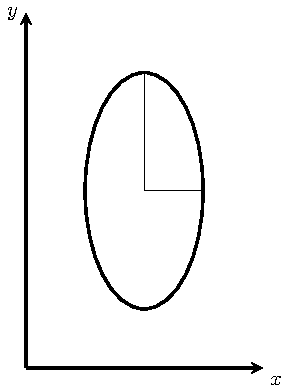
\includegraphics[scale=0.7]{sections/tikz_standalone/ell_13.pdf}\\
     \hline
\end{tabular}
\end{center}
\addtocounter{page}{-2}
\clearpage

\newpage